\section{Umsetzungskonzept für die digitale Transformation}

 Hier sag ich was ich machen werde

\subsection{Repräsentativer Anwendungsfall für die Energiewirtschaft}\label{usecase}

Die verschiedenen Werttreiber und Anforderungen für ein Digitalisierungskonzept unterscheiden sich je nach Unternehmen und Branche.
Für eine erfolgreiche Transformation müssen daher individuelle Anwendungsfälle identifziert werden.
In Anbetracht der Dynamik und des rasanten Tempos, in der neue Technologien entstehen,
ermöglicht ein anwendungsfallbasierter Ansatz eine flexible und agile Anpassung. \citep[S. 31]{Acharya2019}
\\Aus diesen Gründen wird im Folgenden ein repräsentativer Geschäftsprozess für die Energiebranche
und den damit entstehenden Anforderungen dargestellt.
\newline (Hier Bezug auf Motivation für Energiebranche nehmen und anschließend den Geschftsprozess)
ess erläutern.

\subsubsection{Geschäftsprozess}

\subsubsection{Anforderungen}
\begin{itemize}
  \item Aus Requirements Engineering S. 10: Simulation vor Inbetriebnahme, um Fehler in Anforderungsanalyse festzustellen, damit Change Requests gemacht werden können
  \item Bei Anlagen, die mehrere Millionen Euro kosten, sind anders als in Software Mechanik und Elektronik eingebaut. Ein Change Request wäre viel zu teuer
  \item Anforderungsanalyse der Simulation beseitigt die Risiken nicht vollständig, da die Simulation nur so gut ist, wie man sich vorher Gedanken gemacht hat
  \item Welche Anforderungen ergeben sich aus dem Wandel?
  \item Anforderungen wie predictive Maintenance und Bezug auf RAMI 4.0.
  \item SAP als Tool, da Energiesektor hauptsächlich \acf{sapisu}
  \item Industrie 4.0-Komponente (Bitkom s. 52) mit verschiedenen Ebenene
\end{itemize}

\textbf{Anforderungen an Versorgungsunternehmen im Energiesystem der Zukunft \citep[S. 19]{Doleski2016}}

\paragraph{Merkmale von Akteuren in der digitalen Welt}
\begin{itemize}
  \item Allgegenwärtige Informationsverfügbarkeit
  \item Soziale Visualisierung
  \item Absolute Mobilität
  \item Permanente Erreichbarkeit
  \item Lokalisierung
  \item Leistungsfähige Technologien
\end{itemize}

\paragraph{Wesentliche Herausforderungen für Energieunternehmen \citep[S. 21]{Doleski2016}}
\begin{enumerate}
  \item \textbf{Informationsflut}: zunehmendes Informationsangebot kann nicht oder nur bedingt aufgenommen werden
  \item \textbf{Informationsverarbeitung}: zunehmendes Informationsangebot kann nicht zu Wissen verarbeitet werden
  \item \textbf{Informationssysteme}: bestehende Informationssysteme liefern oftmals keine relevanten Informationen für die Unternehmensführung
\end{enumerate}
%


\paragraph{Einige Anforderungen an Versorgungsunternehmen}
Die Anforderungen sollen sich nur auf die Befähiger/Enabler sowie die Prozesse der Energieunternehmen beziehen
\begin{enumerate}
  \item Im Wettbewerb um geeignete Fachkräfte und Digital Natives bestehen $[Enabler]$
  \item Aufbau eines leistungsfähigen Informationsmanagements zur Speicherung, Verarbeitung und Auswertung sehr großer Datenmengen in Echtzeit $[Enabler]$
  \item Big Data beherrschen und innovative technische Lösungen anbieten $[Enabler]$
  \item Image eines verantwortungsbewusst handelnden Unternehmens schaffen und glaubhaft leben $[Enabler]$
  \item Kosteneffizient und professionell handeln $[Prozesse]$
  \item Veränderung von Organisation und Betriebsprozessen zügig vorantreiben $[Prozesse]$
  \item Alle Abläufe müssen modernen Datensicherheitsanforderungen entsprechen $[Prozesse]$
  \item uvm
\end{enumerate}


\subsection{Systementwurf und -analyse}
Systementwurf: Hier mein angepasstes Architekturmodell -> konkretes Architekturmodell mit Sensoren, Edge Device (RPI), SCP (CF) mit Leo IoT Services; AWS SNS mit API-Schnittstellen
\\Hier irgendwo auch anmerken in Bezug auf 2.3.3 SAP Leonardo und in der Evaluation ausführlicher vllt, dass zwar der Mehrwert in kombinierter Anwendung besteht, man hier aufgrund einer prototypischen Implementierung und es Bezugs auf IoT nur auf ein Leo-Produkt bezogen wird

\subsubsection{Systemarchitektur}

SOA - Service Orientierte Architektur
\begin{figure}[H]
    \centering
    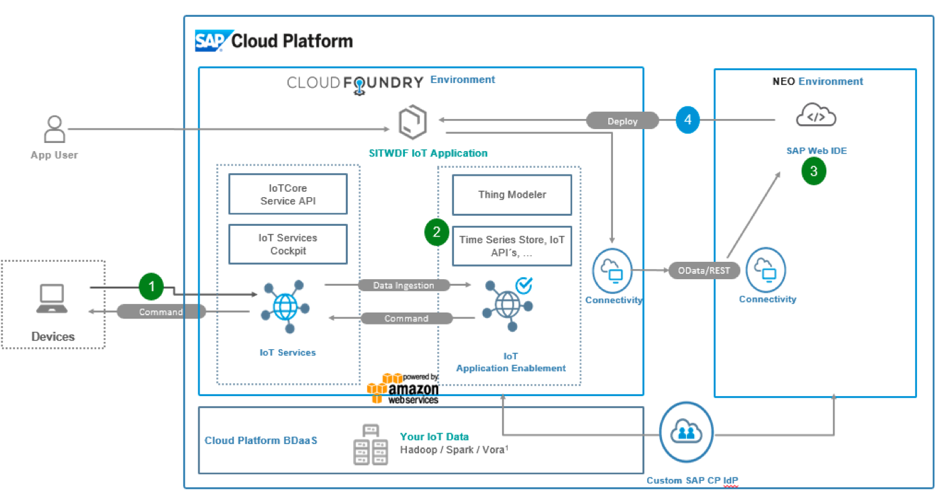
\includegraphics[width=1.0\linewidth]{pictures/sap_architecture}
    \caption[Referenzarchitektur von SAP]{Architektur von SAP \citep{Ganz2019}}
    \label{fig:filename_without_extension}
\end{figure}


\subsubsection{REST API}

\subsubsection{Edge-Processing}

\subsubsection{Destinations}
Destinations: Warum braucht man Destinations und welche man benötigt (SNS),  wenn man kommunizieren will mit
Externe Services wie AWS SNS
Interne Kommunikation der SCP CF und NEO
Communication zwischen Cloud Services AWS SNS und SAP Leonardo

\subsubsection{Message Processing}
Leonardo IoT, SQL Kafka: Ich hab Leonardo IoT benutzt (in prototype erwähnen)

\subsubsection{Sicherheit}
OAuth, SSL/TLS, SAML 2.0: erklären, was SAP und AWS auch eventuell haben

\subsection{Prototypische Implementierung des Anwendungsfalls}
Angewandtes/angepasstes System-Modell
pro Schritt benutztes Sicherheitstechnologie erklären/erwähnen

im Modell auch Schnittstellen, z.B. für SAP Integration, HANA, Leonardo Blockchain und Machine Learning, um zu verdeutlichen, dass die Anforderungen zur sowohl vertikalen (SAP Integration) und horizontalen (Blockchain) erfüllt werden können

\subsubsection{Anbindung der Sensoren an das Edge-Gerät}

\subsubsection{Geräteverwaltung}
mit SAP Cloud Platform Internet of Things und Device Model hier erstellen und als Bild einfügen und außerdem
zunächst auf Tenants und User eingehen und Einrichtungs des Services generell erklären mit eventuell den Message Processings
und Gateways etc

\subsubsection{Einrichtung der Gateway-Edge}

\subsubsection{Senden der Daten an die Cloud}

\subsubsection{Erstellen des digitalen Zwillings}

\subsubsection{Visualisierung mit einer UI5-Applikation}

\subsubsection{Benachrichtigung mit AWS SNS-Server}

\subsubsection{Events generieren mit NodeJs}

\newpage
